
\chapter{Results}
The goal of this thesis was to improve the session-based recommendation system using product embeddings.
From the previous chapter it is evident that this approach did not work as intended.
There are mainly two interesting factors about the measurements in the experiments:
\par
First, the user-layer does not seem to improve the performance, depending on the configuration even produces worse results than unpersonalized session-based recommendations.
The authors of~\cite{hierarchical} found that the performance of the model depends strongly on the user history length.
In their case however, the user-level GRU still improves the performance, even for short user histories.
The main difference between the datasets used in~\cite{hierarchical} and the datasets used in this work is the distribution of the lengths of the sessions.
The datasets in~\cite{hierarchical} in general have less sessions that are longer.
Considering the type of datasets used this is reasonable.
In~\cite{hierarchical}, the authors used two datasets, one dataset comes from XING, a social network for professionals similar to LinkedIn, the second dataset comes from a proprietary video platform similar to YouTube.
The fundamental difference between the afromentioned dataset and the one used in this work is the possible entrypoints to the services.
Both, XING and the video platform, offer a service which is in a way self-contained.
On both services, the user is provided with everything that is needed in the same platform; searching for jobs and connecting with colleagues etc. can all be done in the same session.
Additionally, there is a limited number of entrypoints to these systems.
For an online store the conditions are different.
Many users come through different entrypoints to the online store, such as Google searches, ads or price comparison pages.
A bounce rate analysis shows that 46\% of users arriving on the product detail page leave the site without accessing any other pages on the platform, in other words the users access the online-store for researching product information, but not for browsing.
Each of these visits still produced a session, which would explain the shorter sessions in our dataset.
Even though the user can be identified when looking at one product, little information can be transferred to the next session.
In addition, there are many users who only have few sessions.
\begin{figure}[t]
	\centering
	\captionsetup{width=0.8\textwidth}
    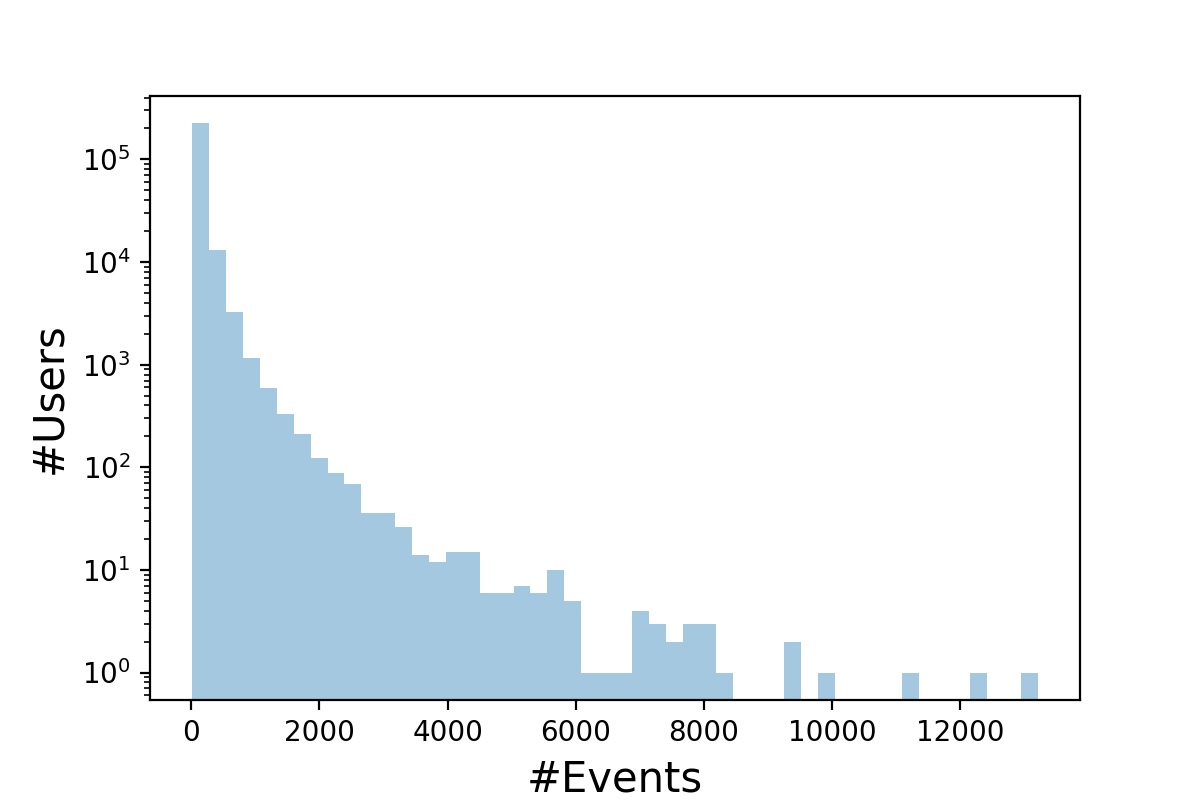
\includegraphics[width=\textwidth]{histo_user_visits.png}
    \caption{Distribution of the number of visits per user (log-scale)}
    \label{fig:histo_user_events}
\end{figure}
Figure~\ref{fig:histo_user_events} illustrates the distribution of the number of visits per user.
What can be seen in the histogram is a phenomenon called \emph{the Long Tail} in the context of web analytics.
There is a very high proportion of users which produce few datapoints, whereas there is a long tail in the distribution, where some users produce extremely many events.
Thus, the information that can be extracted from the majority of users is rather limited.
Of the approximately 250K users there are about 170K users that produced at most 100 events in total across all sessions.
This would explain the limited amount of cross session information we can learn when adding the user-level GRU.
This leads to the fact that the user embedding will not change much from its initial random intitialization, effectively changing nothing about the model, since without the user layer, a session would also be randomly initialized.
\par
The second factor is that the product embedding greatly worsens the results in the offline as well as the online setting.
As explained above, the reason lies in the Long Tail phenomenon, as illustrated in figure~\ref{fig:histo_product_events}.
Of the approximately 470K products, about 320K have at most 100 events recorded.
\begin{figure}[t]
	\centering
	\captionsetup{width=0.8\textwidth}
    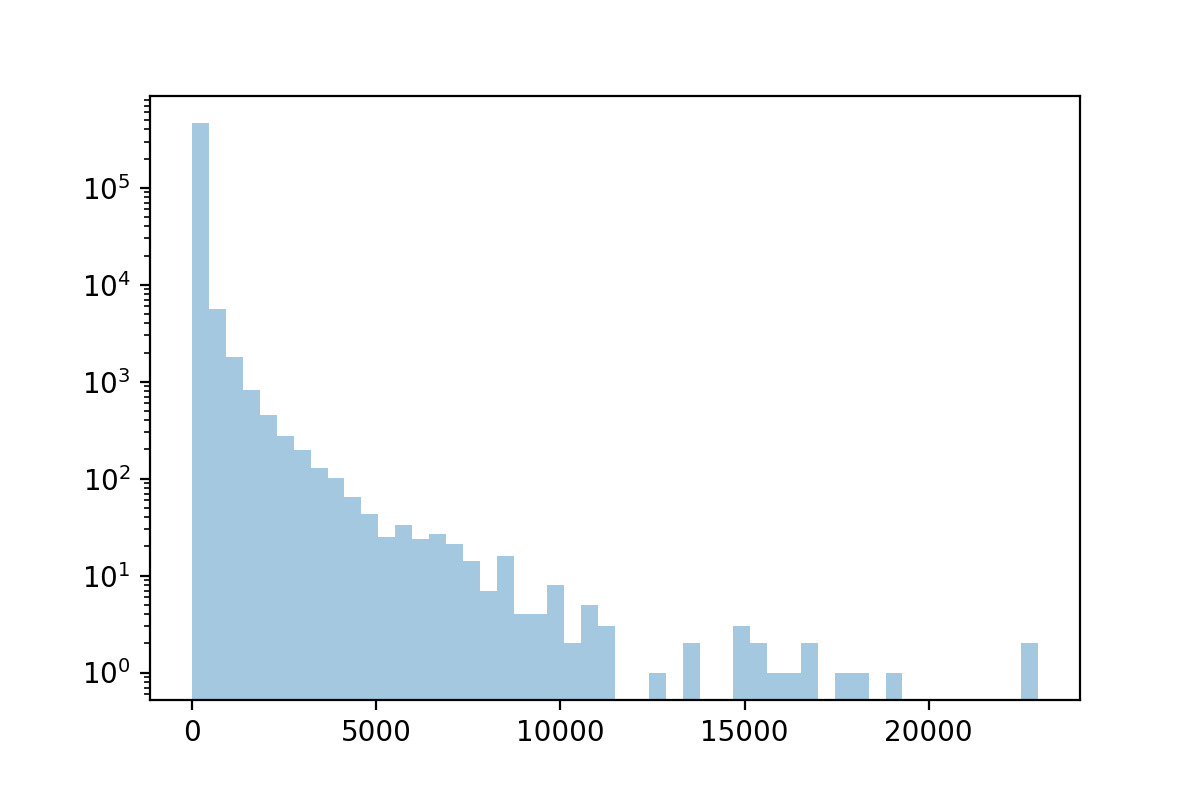
\includegraphics[width=\textwidth]{histo_product_visits.png}
    \caption{Distribution of the number of visits per product (log-scale)}
    \label{fig:histo_product_events}
\end{figure}
\begin{figure}[t]
	\centering
	\captionsetup{width=0.8\textwidth}
    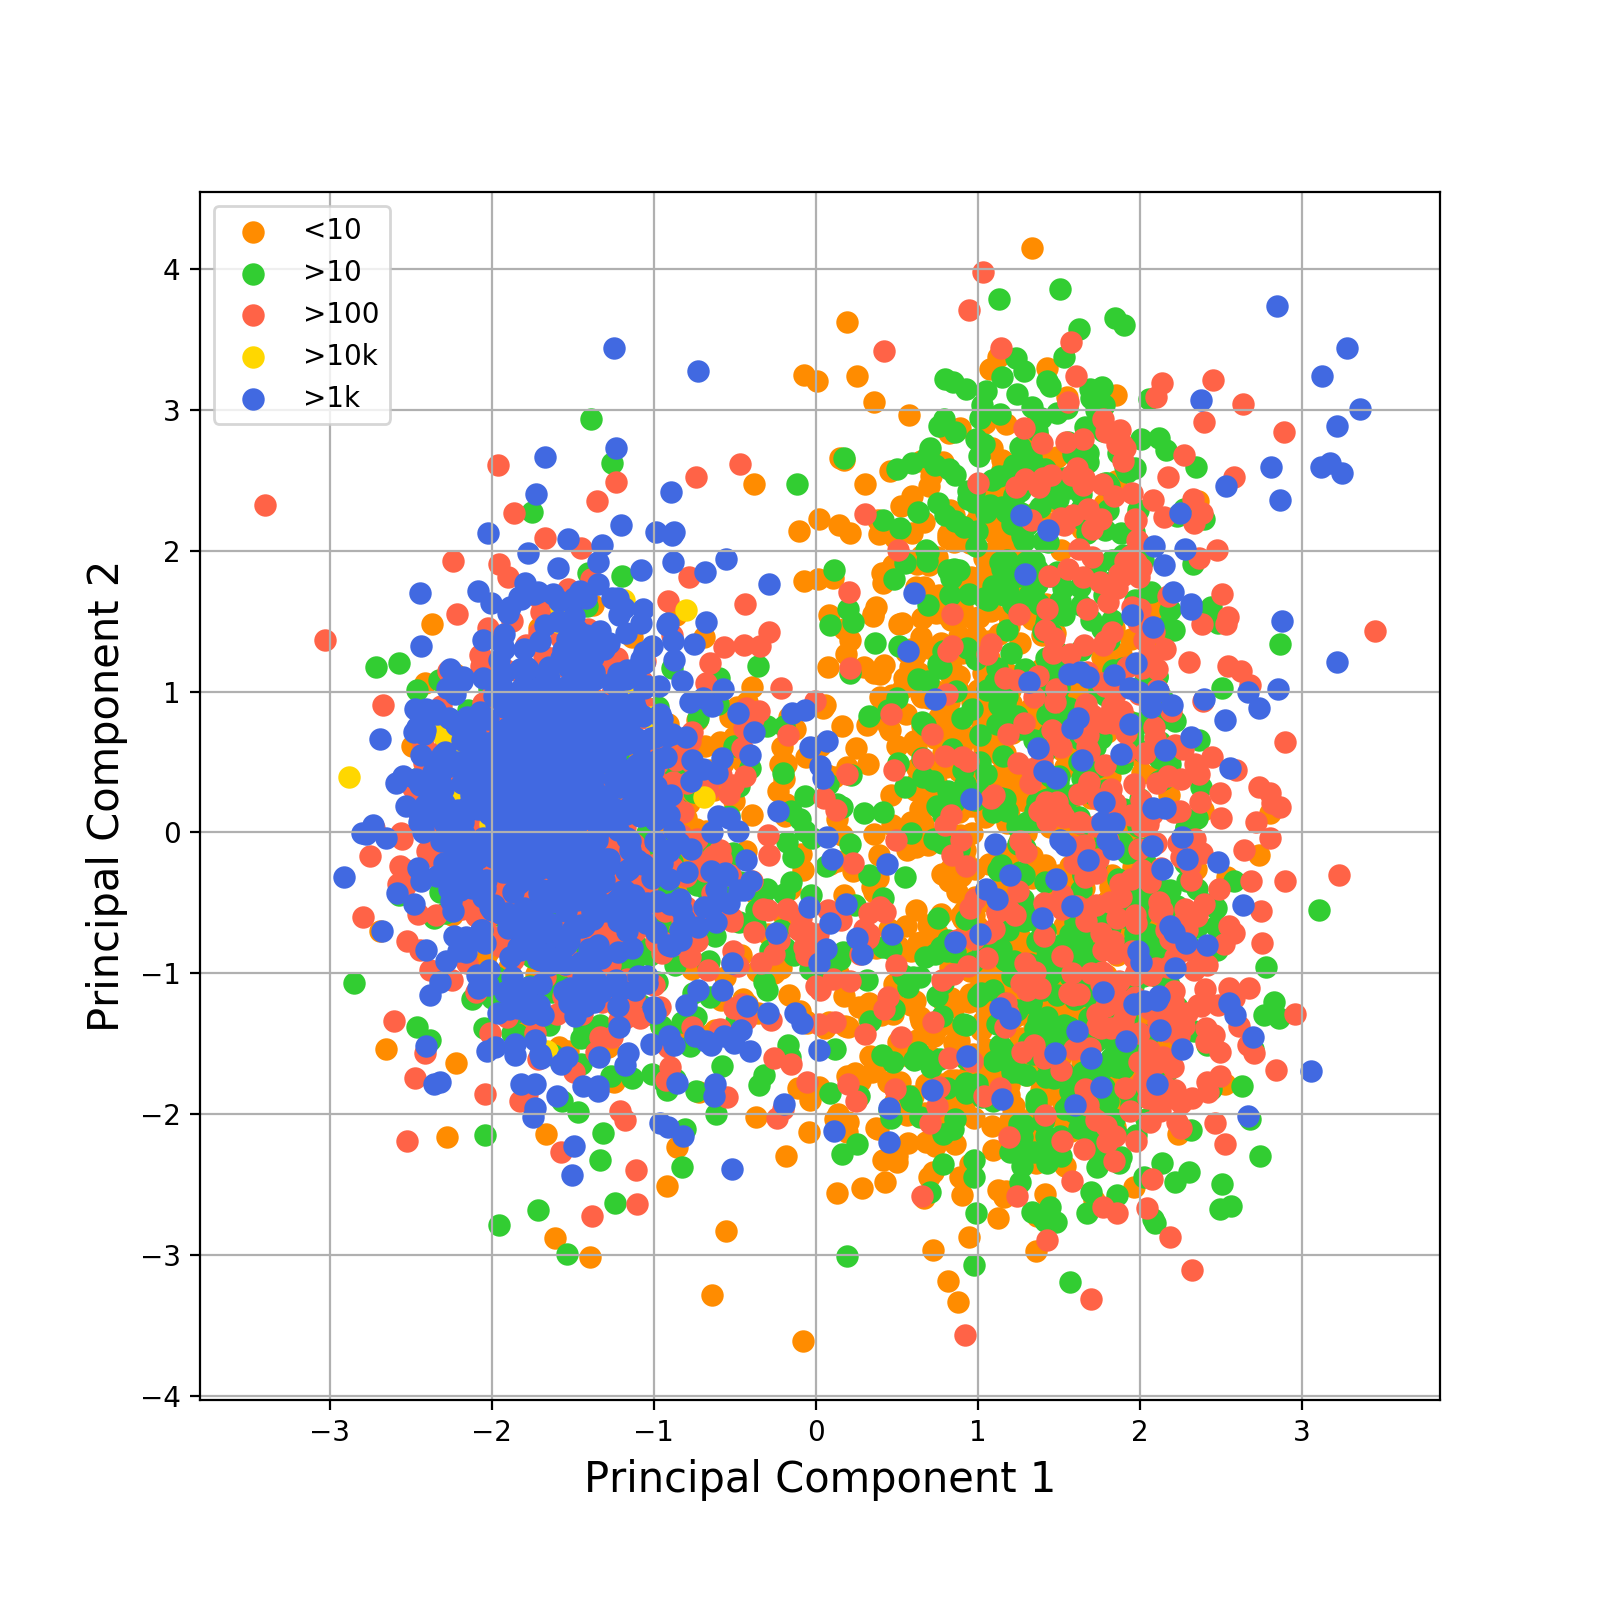
\includegraphics[width=\textwidth]{products_pca.png}
    \caption{PCA of product embeddings}
    \label{fig:products_pca}
\end{figure}
In figure~\ref{fig:products_pca}, we can see a PCA analysis of the product embeddings.
As can be seen in the PCA, there is a separation of datapoints in the first principal component.
\begin{figure}[t]
	\centering
	\captionsetup{width=0.8\textwidth}
    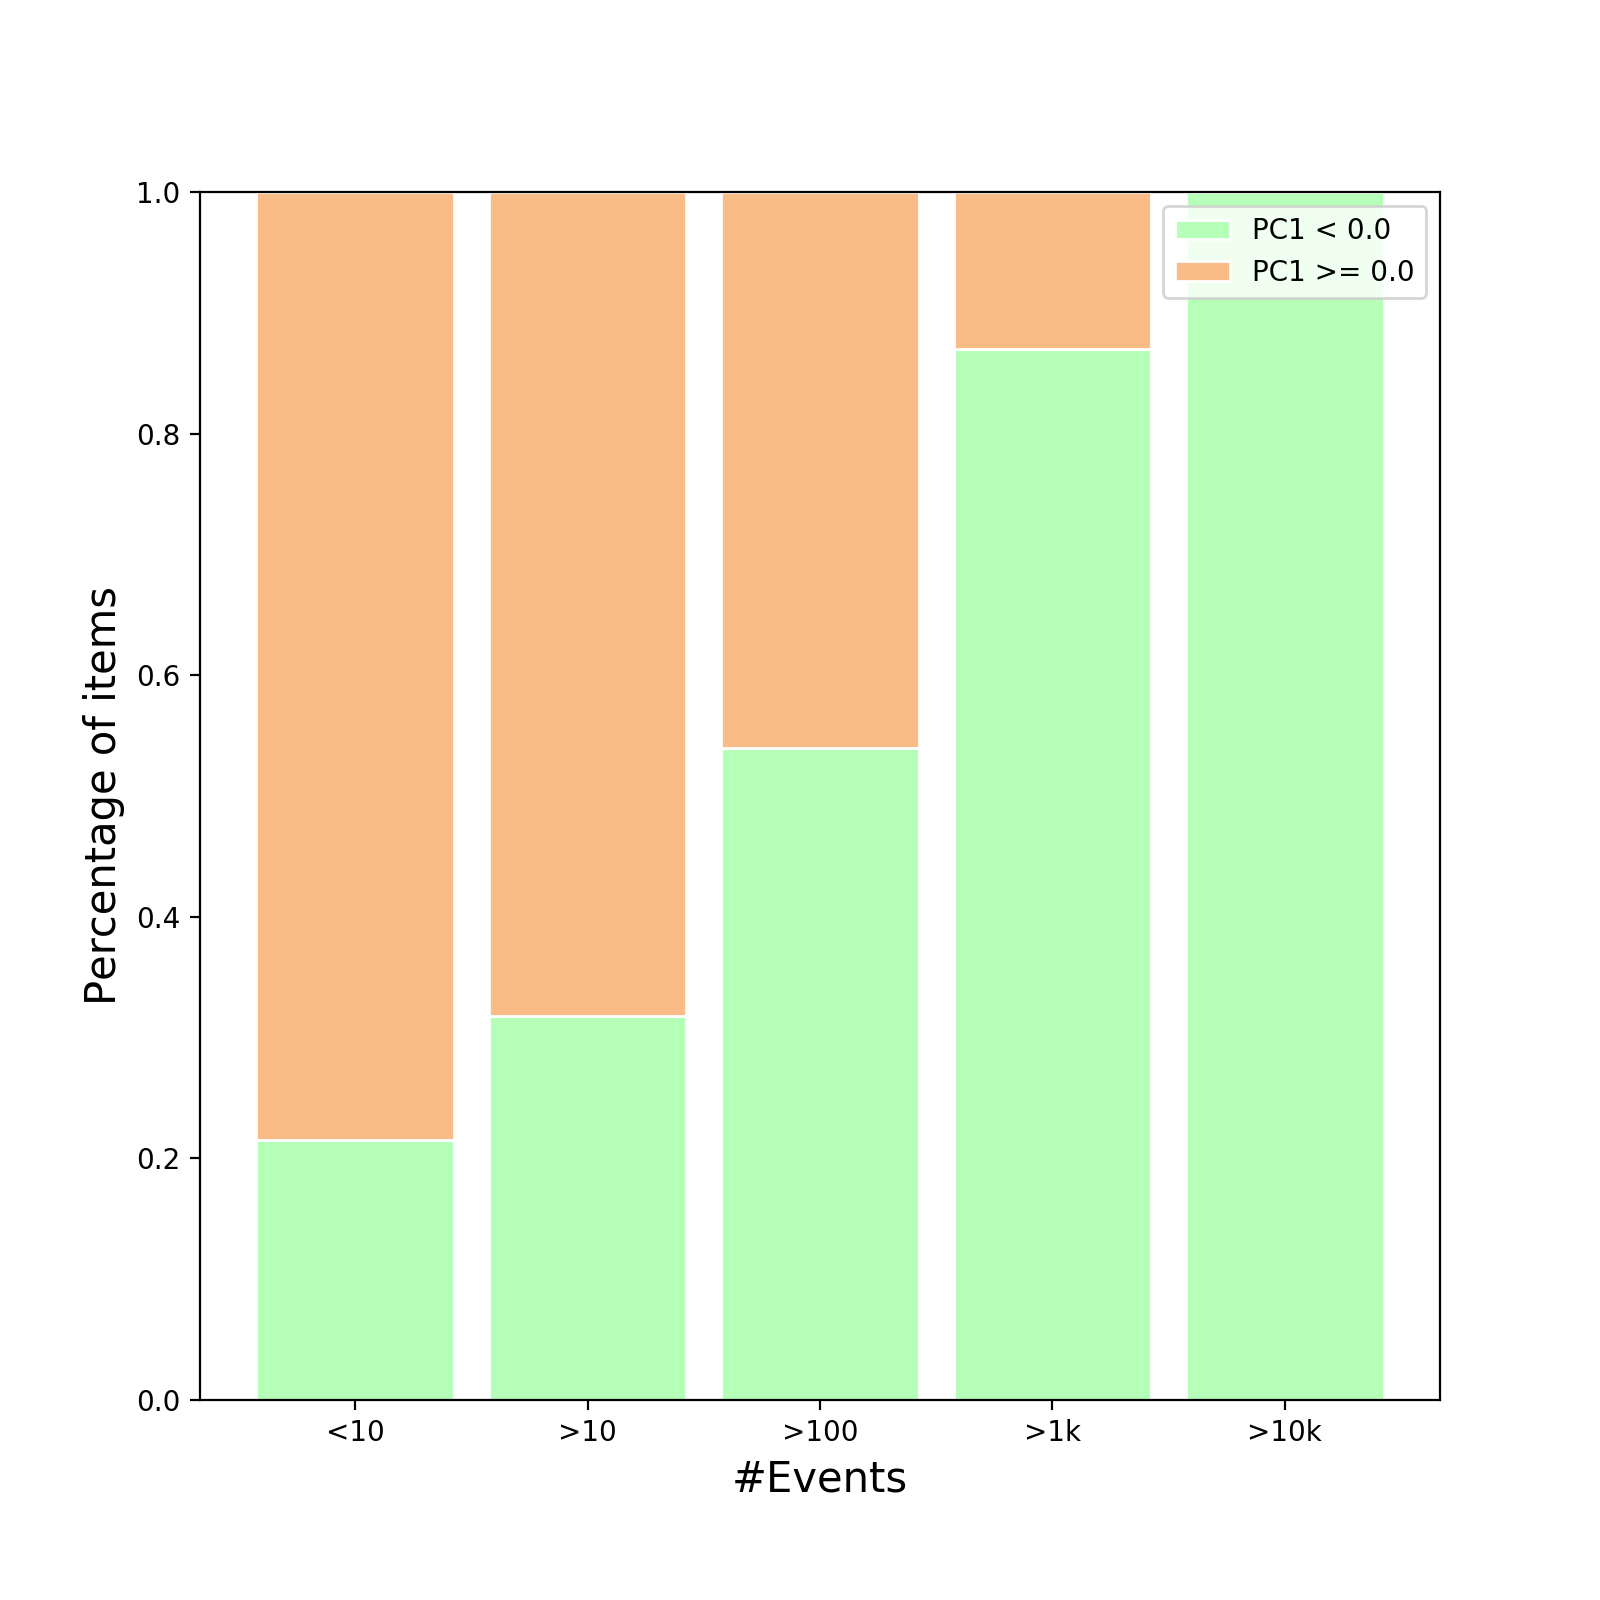
\includegraphics[width=\textwidth]{products_pca_groups.png}
    \caption{Value of PC1}
    \label{fig:products_pca_groups}
\end{figure}
Figure~\ref{fig:products_pca_groups} shows the percentage of datapoints that have the first principal component smaller than 0, grouped by the number of events per product.
As a consequence, the products that generate a lot of events can clearly be separated from the ones producing few events.
This again signifies that, the majority of the product embeddings does not move much from the initial random initialization, since the majority of the products have less than 100 events.
Therefore it is possible that for example a dining table with very few visits is very similar to a shoe with few visits, since both vectors are initialized uniformly at random drawing values from the same distribution.
The problem with this is the signal that is propagated to the GRU:
When using the one-hot encoding, there is always a clear signal which product was the one that was viewed, with the product embedding this is not the case.
Therefore, the network in many cases, basically receives random noise as an input, not being able to produce something else in the output layer.
This has the effect that the predictions in the models using the product embeddings are often the same, recommending items that are viewed many times, but are not a good recommendation based on the currently active item.
\par
In conclusion, it can be said that the sesssion-based approach clearly works.
Even if it does not match the performance of a commercial product, it performs better than more classical approaches to recommendation.
However, personalizing these recommendations turns out to be more difficult than initially thought.
It greatly depends on the number of events produced by each user.
Therefore, it might make sense to focus on personalizing the experience for the subset of users that actually produce enough events.
The same applies to the introduction of product embeddings; the product embeddings have to be of excellent quality such that the network can interpret the signal correctly.
At least the properties of the dataset have a large influence on the success of both the personalization of the recommendations as well as the usage of product embeddings.
\par
A future improvement of this work would be the use of transfer learning.
If the currently active item is an item with few events, a similar item with more events could be used as a replacement for the basis for the recommendation, which would require a secondary similarity measure.
It would also be useful to improve the product embedding.
In~\cite{content2vec} a model is introduced which, in addition to meta information, also takes into account images of a product and its textual description.
Another approach to improving the product embedding could be to parametrize the distribution for the initialization of the vectors to some side-information.
This would remove the issue that very dissimilar products have close embeddings.
Finally another improvement that could be explored is to not only model the sequence of product detail pages, but all the different types of pages in such an online store.
This would give the system the ability to recommend review articles or categories for the user to explore.